\documentclass[aps,onecolumn,11pt]{revtex4}
\usepackage{graphicx}
\usepackage{amssymb,amsfonts,amsmath,amsthm}
\usepackage{chemarr}
\usepackage{bm}
\usepackage{pslatex}
\usepackage{xfrac}
\usepackage[dvipsnames]{xcolor}
\usepackage{bookman}
\usepackage{dsfont}
%\usepackage{mathptmx}
%\usepackage{hyperref}
%\usepackage{rotating}
\usepackage{fancybox}

\newcommand{\mychem}[1]{\mathtt{#1}}
\newcommand{\myconc}[1]{\big[#1\big]}

\newcommand{\Faraday}{\mathcal{F}}
\newcommand{\spLi}[1]{{\!~^{#1}\mychem{Li}}}
\newcommand{\Li}[1]{\myconc{\spLi{#1}}}
\newcommand{\spproton}{\mychem{H}}
\newcommand{\proton}{\myconc{\spproton}}

\newcommand{\deltaLi}{\delta\!\!\spLi{7}}
\newcommand{\myleak}[1]{\left.{#1}\right\vert_{\mathrm{leak}}}
\newcommand{\myout}[1]{{#1}_{\mathrm{out}}}
\newcommand{\LiOut}[1]{\myout{\Li{#1}}}
\newcommand{\spLiOut}[1]{\myout{\spLi{#1}}}

\newcommand{\myrotate}[2]{\rotatebox[origin=c]{#1}{#2}}

\newcommand{\mytrn}[1]{{#1}^{\!\mathsf{T}}}
\newcommand{\mymat}[1]{{\bm{#1}}}
\newcommand{\mydet}[1]{{\left|{#1}\right|}}

\usepackage{ifthen}


\newcommand{\LiAll}{\Lambda}
\newcommand{\LiAllOut}{\myout{\LiAll}}
\newcommand{\deltaLiOut}{\myout{\deltaLi}}
\newcommand{\inpLi}[1]{\text{+}\spLiOut{#1}}
\newcommand{\outLi}[1]{\text{-}\spLiOut{#1}}

\newcommand{\mycolor}[2]{\ifthenelse{\equal{#1}{6}}{{\color{Red}#2}}{{\color{Green}#2}}}

\DeclareMathOperator\erf{erf}
\newcommand{\pH}{\ensuremath{\mathrm{pH}}}
\newcommand{\NHE}[1]{\ensuremath{\mathrm{NHE}_{#1}}}

\newcommand{\todo}[1]{\framebox{#1}}

\begin{document}
\title{Lithium Isotopic Separation:\\ From Electroosmosis to NHE Cooperativity}
\maketitle
%\tableofcontents

\section{Description}
\subsection{Isotopic Separation}
We have two species $\spLi{6}$ and $\spLi{7}$ and a solution can be defined by the isotopic 
separation:
\begin{equation}
	\deltaLi = 10^3 \left[ 
	\dfrac{
	\left(\dfrac{\Li{7}}{\Li{6}}\right)
	}
	{
	\left(\dfrac{\Li{7}}{\Li{6}}\right)_{standard}
	}
	- 1 \right]
\end{equation}
and alternatively:
\begin{equation}
	\left(\dfrac{\Li{7}}{\Li{6}}\right) = \lambda_s \left[ 1+10^{-3} \deltaLi \right]
\end{equation}
where we are using:
\begin{equation}
	\rho_s = \left(\dfrac{\Li{7}}{\Li{6}}\right)_{standard} %=  12.0192
\end{equation}
We define:
\begin{equation}
	\LiAll = \Li{6}+\Li{7}
\end{equation}
and we obtain the relations:
\begin{equation}
\left\lbrace
\begin{array}{rcl}
\Li{6} & = & \dfrac{1}{1+\rho_s[1+10^{-3}\deltaLi]} \LiAll \\
\\
\Li{7} & = &  \dfrac{\rho_s[1+10^{-3}\deltaLi]}{1+\rho_s[1+10^{-3}\deltaLi]}\LiAll\\
\end{array}
\right.
\end{equation}
\subsection{Numerical Values}
For the current experiments:
\begin{equation}
\left\lbrace
\begin{array}{rcl}
	\rho_s   & = & 12.0192\\
	\deltaLiOut & = & 14.57\\
	\LiOut{6}   & = & \epsilon_6 \LiAllOut, \;\;\epsilon_6\simeq 0.076\\
	\LiOut{7}   & = & \epsilon_7 \LiAllOut, \;\;\epsilon_7\simeq 0.924\\
\end{array}
\right. 
\end{equation}
If we use the normalised values:
\begin{equation}
\label{eq:beta}
\left\lbrace
\begin{array}{rcl}
	\beta_6 & = & \dfrac{\Li{6}}{\LiOut{6}}\\
	\\
	\beta_7 & = & \dfrac{\Li{7}}{\LiOut{7}}\\
	\\
	\dfrac{\beta_7}{\beta_6} & = & \dfrac{\left[1+10^{-3}\deltaLi\right]}{\left[1+10^{-3}\deltaLiOut\right]}\\
	\\
	\deltaLi & = & 10^3 \left( \left[1+10^{-3}\deltaLiOut\right]\dfrac{\beta_7}{\beta_6} -1 \right)\\
\end{array}
\right.
\end{equation}


\section{Electro-osmotic Intake}
\subsection{Goldman-Hodgkins-Katz (GHK) Flux}
The two species $\spLi{6}$ and $\spLi{7}$ that may leak through the membrane by borrowing some ionic channels:
\begin{equation}
\left\lbrace
\begin{array}{rcl}
	\Theta    & = & e^{\dfrac{-\Faraday V_m }{RT}} \\
	\partial_t \myleak{\Li{u}} & = & k_u \left( \Theta \LiOut{u} - \Li{u}\right)\\
\end{array}
\right.
\end{equation}
According to the GHK theory, both $k_6$ and $k_7$ are the whole cell permeability to $\spLi{6}$ and $\spLi{7}$ respectively,
and should depend on the potential. But in any case, this permeability arises from a diffusive process, and we expect the ratio to be constant:
\begin{equation}
\label{eq:sigma}
	\dfrac{k_6}{k_7} \simeq \sigma = 1.00229
\end{equation}

\subsection{Potential Regulation}
One the one hand, since this intake is not electroneutral, it shall produces a drift in the cell polarisation. But on the other hand, the cell is able to regulate its potential 
by a mechanism that we shall simply model by a first order return function:
\begin{equation}
	\partial_t V_m = \gamma \left( \partial_t \myleak{\Li{6}} + \partial_t \myleak{\Li{7}} \right) + k_m \left(V_0-V_m\right)
\end{equation}

\section{Catalytic One-Layer NHE}

\subsection{Kinetic Scheme}
We use $E$ to describe the $NHE$ state.
{
\Large
\begin{equation}
\boxed{
\begin{array}{ccccc}
 & & E_{06}  &  & \\
 &  \mycolor{6}{\myrotate{45}{$\xrightleftharpoons[\outLi{6},\;d_{06}]{+\spLiOut{6},\;a_{06}}$}} &   & \mycolor{6}{\myrotate{-45}{$\xrightarrow[-\spLi{6}]{+ \spproton, \; k^p_6}$}} &  \\
E_{00}  &  & \xleftarrow{\text{ recycling } k_h } &   & E_{0H} \\
  & \mycolor{7}{\myrotate{-45}{$\xrightleftharpoons[\outLi{7},\;d_{07}]{+\spLiOut{7},\;a_{02}}$}} &   & \mycolor{7}{\myrotate{+45}{$\xrightarrow[-\spLi{7}]{+ \spproton, \; k^p_7}$}} & \\
 & & E_{07} & & \\
 \end{array}
 }
\end{equation}
}

\subsection{Differential Equations}
The evolution of the species and the total enzyme conservation are described by:
\begin{equation}
\left\lbrace
\begin{array}{rcl}
\partial_t E_{00} & = & D_{06}-A_{06} + D_{07}-A_{07} + v_h\\
\partial_t E_{06} & = & -D_{06}+A_{06} -v^p_6 \\
\partial_t E_{07} & = & -D_{07}+A_{07} -v^p_7\\
\partial_t E_{0H} & = & v^p_6 + v^p_7 - v_h\\
\mathsf{E}       & = & E_{00}+E_{01}+E_{02} + E_{0H} = E_{0H} + {\displaystyle \sum_{x\leq y\leq 1} E_{xy}}\\
\end{array}
\right.
\end{equation}
with the kinetic terms:
\begin{equation}
\left\lbrace
\begin{array}{rcl}
A_{06} &= &a_{06} E_{00} \LiOut{6}\\
A_{07} &= &a_{07} E_{00} \LiOut{7}\\
D_{06} &= &d_{06} E_{06}\\
D_{07} &= &d_{07} E_{07}\\
v^p_6  &=& k^p_6 E_{06} \proton\\
v^p_7  &=& k^p_7 E_{07} \proton\\
v_h    &=& k_h   E_{0H}
\end{array}
\right.
\end{equation}

\subsection{Pre-Equilibria Hypothesis}
\subsubsection{Lithium Intake Rate}
We assume that the reversible forms some pre-equilibria before allowing the irreversible reactions to occur.
\begin{equation}
\left\lbrace
\begin{array}{rcll}
	E_{06}^\star & = & \dfrac{a_{06}}{d_{06} } E_{00} \LiOut{6} & = J_6 E_{00} \LiOut{6}\\
	\\
	E_{07}^\star & = & \dfrac{a_{07}}{d_{07}  } E_{00} \LiOut{7} & = J_7 E_{00} \LiOut{7}\\
\end{array}
\right.
\end{equation}


Finally:
\begin{equation}
\mathsf{E} = E_{00}\left(1+J_6\LiOut{6}+J_7\LiOut{7}\right) + E_{0H} \Leftrightarrow E_{00} = \dfrac{\mathsf{E}-E_{0H}}{1+J_6\LiOut{6}+J_7\LiOut{7}}
\end{equation}
and:
\begin{equation}
\left\lbrace
\begin{array}{rcl}
	E_{06}^\star & = & \dfrac{J_6\LiOut{6}}{1+J_6\LiOut{6}+J_7\LiOut{7}} \left(\mathsf{E}-E_{0H}\right)\\
	\\
	E_{07}^\star & = & \dfrac{J_7\LiOut{7}}{1+J_6\LiOut{6}+J_7\LiOut{7}} \left(\mathsf{E}-E_{0H}\right)\\
\end{array}
\right.
\end{equation}
so that we have the three equations:
\begin{equation}
\left\lbrace
\begin{array}{rcl}
	\partial_t \Li{u}  & = & v^p_u +\partial_t \myleak{\Li{u}}  = \dfrac{k^p_u J_u \LiOut{u}}{1+\sum_v J_v \LiOut{v}} \left(\mathsf{E}-E_{0H}\right) \proton + k_u \left( \Theta \LiOut{u} - \Li{u}\right) \\
	\\
	\partial_t E_{0H} & = & -k_h E_{0H} + \dfrac{\sum_v k^p_u J_u \LiOut{u}}{1+\sum_v J_v \LiOut{v}} \left(\mathsf{E}-E_{0H}\right) \proton \\
\end{array}
\right.
\end{equation}
\subsubsection{Normalisation}
We use the definitions of Eq \eqref{eq:beta} and the following:
\begin{equation}
\left\lbrace
\begin{array}{rcl}
%	\LiOut{u} & = & \epsilon_u \LiAllOut\\
%	\\
%	\beta_u & = & \dfrac{\Li{u}}{\LiOut{u}}\\
%	\\
	\alpha  & = & \dfrac{E_{0H}}{\mathsf{E}}\\
	\\
	J_0 & = & \epsilon_6 J_6  + \epsilon_7 J_7 \\
\end{array}
\right.
\end{equation}

We are left with the four equations:
\begin{equation}
\left\lbrace
\begin{array}{rcl}
\partial_t V_m & = & \gamma\LiAllOut \left[\sum_x \epsilon_x k_x \left( \exp\left[ -\frac{\Faraday V_m}{RT}\right] -\beta_x \right)  \right] + k_m\left(V_0-V_m\right)\\
\\
\partial_t \beta_u & = & \mathsf{E} \left[\dfrac{k^p_u J_u}{1+J_0 \LiAllOut}\right] \left(1-\alpha\right) \proton
	 + k_u \left( \exp\left[-\frac{\Faraday V_m}{RT}\right] - \beta_u\right),\;\;u\in\lbrace6,7\rbrace\\
\\
\partial_t \alpha  & = &  -k_h\alpha + \LiAllOut \left[\dfrac{ \sum_v k^p_v \epsilon_v J_v}{1+J_0\LiAllOut}\right] \left(1-\alpha\right) \proton\\
\end{array}
\right.
\end{equation}

\subsubsection{Initial Isotopic Separation}
The evaluation of the initial yields:
\begin{equation}
\label{eq:level1}
	\left(\dfrac{\beta_7}{\beta_6}\right)^\varnothing \simeq \left(\dfrac{\partial_t \beta_7}{\partial_t\beta_6}\right)^\varnothing
	= \dfrac{\mathsf{E} \left[\dfrac{k^p_7 J_7}{1+J_0 \LiAllOut}\right] \proton_0 + k_7  \Theta_0
	}
	{
	\mathsf{E} \left[\dfrac{k^p_6 J_6}{1+J_0 \LiAllOut}\right] \proton_0 + k_6  \Theta_0
	}
\end{equation}
Let us define:
\begin{equation}
	\kappa = \dfrac{k^p_6 J_6}{k^p_7 J_7}, \;\; \phi = \dfrac{ \mathsf{E} \proton_0 }{ k_7  \Theta_0 } \left[\dfrac{k^p_7 J_7}{1+J_0 \LiAllOut}\right] 
\end{equation}
to obtain:
\begin{equation}
	\left(\dfrac{\beta_7}{\beta_6}\right)^\varnothing = \dfrac{1+\phi}{\sigma+\phi\kappa}
\end{equation}
We see that for a catalytic speedup $\kappa$ greater than the diffusive speedup $\sigma$, we reach some higher isotopic separations (lower $\deltaLi$), depending
on the $\phi$ factor, which is experimentally much greater than one.
Nonetheless, the value of $\phi$ is {\bf decreasing} with $\LiAllOut$, meaning that the isotopic separation is decreasing with respect to the total lithium concentration.
Accordingly, we have to derive a higher order model.

\section{Catalytic Two-Layers NHE : Cooperativity}
\subsection{Full Kinetic Scheme}
The cooperative model may be written as the following scheme, with \textit{a priori} no restriction on microscopic values:
{
\Large
\begin{equation}
\boxed{
\begin{array}{ccccccc}
 & &        &                                                  & E_{66} & & \\
 & &        & \myrotate{45}{\mycolor{6}{$\xrightleftharpoons[\outLi{6},\;d_{66}]{\inpLi{6},\;a_{66}}$}} & &  \myrotate{-45}{\mycolor{6}{$\xrightarrow[-\spLi{6}]{+ \spproton, \; k^p_{66}}$}}& \\
 & & E_{06} &  & \xleftarrow{\text{ recycling } k^h_6 } & & E_{6H}\\
 &  \myrotate{45}{\mycolor{6}{$\xrightleftharpoons[\outLi{6},\;d_{06}]{\inpLi{6},\;a_{06}}$}} &   & \myrotate{-45}{\mycolor{7}{$\xrightleftharpoons[\outLi{7},\;d_{67}]{\inpLi{7},\;a_{67}}$}} & & \myrotate{45}{\mycolor{7}{$\xrightarrow[-\spLi{7}]{+ \spproton, \; k^p_{67}}$}}&\\
E_{00} & &  & & E_{67}(=E_{76}) & & \\ 
  & \myrotate{-45}{\mycolor{7}{$\xrightleftharpoons[\outLi{7},\;d_{07}]{\inpLi{7},\;a_{07}}$}} &  & \myrotate{45}{\mycolor{6}{$\xrightleftharpoons[\outLi{6},\;d_{76}]{\inpLi{6},\;a_{76}}$}} & & \myrotate{-45}{\mycolor{6}{$\xrightarrow[-\spLi{6}]{+ \spproton, \; k^p_{76}}$}} & \\
  & & E_{07} &   & \xleftarrow{\text{ recycling } k^h_7 } & & E_{7H}\\
  & &  & \myrotate{-45}{\mycolor{7}{$\xrightleftharpoons[\outLi{7},\;d_{77}]{\inpLi{7},\;a_{77}}$}} & & \myrotate{45}{\mycolor{7}{$\xrightarrow[-\spLi{7}]{+ \spproton, \; k^p_{77}}$}} &\\
  & &  &  & E_{77} & &\\

 \end{array}
 }
\end{equation}
}


\subsection{Differential Equations}
We convert the scheme into a set of differential equations:
\begin{equation}
\left\lbrace
\begin{array}{rcl}
\partial_t E_{00} & = & D_{06}-A_{06} + D_{07}-A_{07}\\
\partial_t E_{06} & = & -D_{06}+A_{06} - A_{66} + D_{66} - A_{67} + D_{67} + v_{6H}\\
\partial_t E_{07} & = & -D_{07}+A_{07} - A_{77} + D_{77} - A_{76} + D_{76} + v_{7H}\\
\partial_t E_{66} & = & A_{66}-D_{66} -v^p_{66}\\
\partial_t E_{67} & = & A_{67}-D_{67} + A_{76}-D_{76} - (v^p_{67}+v^p_{76})\\
\partial_t E_{77} & = & A_{77}-D_{77} - v^p_{77}\\
\partial_t E_{6H} & = & v^p_{66}+v^p_{67} - v_{6H}\\
\partial_t E_{7H} & = & v^p_{77}+v^p_{76} - v_{7H}\\
\mathsf{E}      & = & {\displaystyle \sum_{x\leq y} E_{xy}}+E_{6H}+E_{7H}\\
\end{array}
\right.
\end{equation}
where we build up the terms:
\begin{equation}
\left\lbrace
\begin{array}{rcl}%|rcl}
A_{06}   & = & a_{06} E_{00} \LiOut{6}  \\% & A'_{06}   & = & a_{06}    \alpha_{00} \LiOut{6}\\
A_{07}   & = & a_{07} E_{00} \LiOut{7}  \\%& A'_{07}   & = & a_{07}    \alpha_{00} \LiOut{7}\\
D_{06}   & = & d_{06} E_{06}            \\%& D'_{06}   & = & d_{06}    \alpha_{06}\\
D_{07}   & = & d_{07} E_{07}            \\%& D'_{07}   & = & d_{07}    \alpha_{07}\\
A_{66}   & = & a_{66} E_{06} \LiOut{6}  \\%& A'_{66}   & = & a_{66}    \alpha_{06} \LiOut{6} \\
D_{66}   & = & d_{66} E_{66}            \\%& D'_{66}   & = & d_{66}    \alpha_{66}\\
A_{77}   & = & a_{77} E_{07} \LiOut{7}  \\%& A'_{77}   & = & a_{77}    \alpha_{07} \LiOut{7}\\
D_{77}   & = & d_{77} E_{77}            \\%& D'_{77}   & = & d_{77}    \alpha_{77}\\
A_{67}   & = & a_{67} E_{06} \LiOut{7}  \\%& A'_{67}   & = & a_{67}    \alpha_{06} \LiOut{7}\\
D_{67}   & = & d_{67} E_{67}            \\%& D'_{67}   & = & d_{67}    \alpha_{67}\\
A_{76}   & = & a_{76} E_{07} \LiOut{6}  \\%& A'_{76}   & = & a_{76}    \alpha_{07} \LiOut{6}\\
D_{76}   & = & d_{76} E_{67}            \\%& D'_{76}   & = & d_{76}    \alpha_{67}\\
v_{6H}   & = & k^h_6 E_{6H}             \\%& v'_{6H}   & = & k^h_6    \alpha_{6H} \\
v_{7H}   & = & k^h_7 E_{7H}             \\%& v'_{7H}   & = & k^h_7    \alpha_{7H} \\
v^p_{66} & = & k^p_{66} E_{66} \proton  \\%& v'^p_{66} & = & k^p_{66} \alpha_{66} \proton\\
v^p_{77} & = & k^p_{77} E_{77} \proton  \\%& v'^p_{77} & = & k^p_{77} \alpha_{77} \proton\\
v^p_{67} & = & k^p_{67} E_{67} \proton  \\%& v'^p_{67} & = & k^p_{67} \alpha_{67}\\
v^p_{76} & = & k^p_{76} E_{67} \proton  \\%& v'^p_{76} & = & k^p_{76} \alpha_{67} \proton\\
\end{array}
\right.
\end{equation}
and the different lithium intakes are:
\begin{equation}
\left\lbrace
\begin{array}{rcl}
	\partial_t \Li{6} & = & v^p_{66}+v^p_{76} + \partial_t \myleak{\Li{6}} \\ %& = & \partial_t \myleak{\Li{6}} + \mathsf{E} \left( v'^p_{66}+v'^p_{76}\right) \\
	\\
	\partial_t \Li{7} & = & v^p_{77}+v^p_{67} + \partial_t \myleak{\Li{7}} \\ %& = & \partial_t \myleak{\Li{7}} + \mathsf{E} \left( v'^p_{66}+v'^p_{76}\right)\\
\end{array}
\right.
\end{equation}

\subsection{Algebraic Notations}



We define:
\begin{itemize}
\item the first layer variables:
\begin{equation}
	\vec{E}_1 = \begin{bmatrix}
	E_{06}\\
	E_{07}\\
	\end{bmatrix}
\end{equation}
\item and the second layer variables:
\begin{equation}
	\vec{E}_2 = \begin{bmatrix}
	E_{66}\\
	E_{67}\\
	E_{77}\\
	\end{bmatrix}
\end{equation}
\item the outer concentrations:
\begin{equation}
\label{eq:C}
	\vec{C} = 
	\begin{bmatrix}
	\LiOut{6}\\
	\LiOut{7}\\
	\end{bmatrix}
	=
	\LiAllOut
	\begin{bmatrix}
	\epsilon_6\\
	\epsilon_7\\
	\end{bmatrix}
	=
	\LiAllOut\vec{\epsilon},\;\;
	\mymat{\Delta}_C = 
	\begin{bmatrix}
	C_6 & 0\\
	 0& C_7\\
	\end{bmatrix}
\end{equation}
\item the protonated enzymes:
\begin{equation}
	\vec{E}_H = 
	\begin{bmatrix}
	E_{6H}\\
	E_{7H}\\
	\end{bmatrix}
\end{equation}
\item the algebraic projection terms:
\begin{equation}
	\vec{L}_1 = 
	\begin{bmatrix}
	1\\
	1\\
	\end{bmatrix},\;\;
	\mymat{Q}_1 = 
	\begin{bmatrix}
	1&1\\
	1&1\\
	\end{bmatrix}
\end{equation}

\end{itemize}

\subsection{Second layer as a function of the first layer}

Using the three equations describing the second layer and assuming that the internal pre-equilibria are reached, we find
that the second layer components are bilinear combinations of the first layer components:
\begin{equation}
\boxed{
E_{xy} = <{\vec{C}} \vert \mymat{F_{xy}} \vert \vec{E}_1 > 
}
\end{equation}
with:
\begin{equation}
\left\lbrace
\begin{array}{rcl}
\mymat{F}_{66} & = & 
\begin{bmatrix}
	\dfrac{a_{66}}{d_{66} } & 0 \\
	0 & 0\\
\end{bmatrix} \\
\\
\mymat{F}_{77} & = & 
\begin{bmatrix}
	0 & 0 \\
	0 & \dfrac{a_{77}}{d_{77} }\\
\end{bmatrix}  \\
\\
\mymat{F}_{67} & = & 
\begin{bmatrix}
	0 &\dfrac{a_{76}}{d_{76}+d_{67}}\\
	\dfrac{a_{67}}{d_{76}+d_{67}} & 0\\
\end{bmatrix} \\
\end{array}
\right.
\end{equation}
and the second layer mass as a function of the first layer values is:
\begin{equation}
E_{66} + E_{67} + E_{77} = <{\vec{C}} \vert \mymat{F} \vert \vec{E}_1 >, \;\;
 \mymat{F} 
 =  \mymat{F}_{66} + \mymat{F}_{67}  + \mymat{F}_{77}
\end{equation}

We also get a compact writing of the lithium intake:
\begin{equation}
\left\lbrace
\begin{array}{rcl}
	\partial_t \Li{6} & = & <\vec{C}|\mymat{G}_6|\vec{E}_1> \proton+ k_6\left(\Theta \LiOut{6} - \Li{6}\right)\\
	\mymat{G}_6 &= & k^p_{66} \mymat{F}_{66} + k^p_{67}\mymat{F}_{67}	\\
	\\
	\partial_t \Li{7} & = & <\vec{C}|\mymat{G}_7|\vec{E}_1> \proton + k_7\left(\Theta \LiOut{7} - \Li{7}\right)\\
	\mymat{G}_7 & = & k^p_{77} \mymat{F}_{77} + k^p_{76}\mymat{F}_{67} \\
\end{array}
\right.
\end{equation}


\subsection{First layer as a function of the external components}
We define the following constants:
\begin{equation}
\left\lbrace
\begin{array}{rcl}
\mymat{\Delta}_A &= &\begin{bmatrix}
a_{06} & 0 \\
0 & a_{07} \\
\end{bmatrix}\\
\\
\mymat{\Delta}_D & = & 
\begin{bmatrix}
d_{06} & 0 \\
0 & d_{07} \\
\end{bmatrix} \\
\\
K_6 & = & \dfrac{1}{d_{07}d_{06}}  \dfrac{a_{76}d_{67}}{d_{67}+d_{76}} \\
\\
K_7 & = &  \dfrac{1}{d_{06}d_{07}} \dfrac{a_{67}d_{76}}{d_{67}+d_{76}} \\
\\
\mymat{\Delta}_K & = & \begin{bmatrix} K_6 & 0 \\ 0 & K7 \\ \end{bmatrix}
\end{array}
\right.
\end{equation}
Leading to the algebraic expressions:
\begin{equation}
\left\lbrace
\begin{array}{rcl}
W_1 & = & 1 +  <\vec{L}_1| \mymat{\Delta}_K \mymat{\Delta}_D | \vec{C}> = 1+ <\vec{L}_w|\vec{C}> \\
\\
\mymat{M_1} & = & \mymat{\Delta}_D^{-1} + \mymat{\Delta}_C \mymat{\Delta}_K \mymat{Q}_1 \\
\end{array}
\right.
\end{equation}
Thus, the first layer expression as a function of the entry layer is
\begin{equation}
\boxed
{
W_1 \vec{E}_1  =  E_{00} \mymat{M}_1  \mymat{\Delta}_A \vec{C}
}
\end{equation}

\subsection{Using Mass Conservation to compute the entry layer}
We expand and factorise:
\begin{equation}
\left\lbrace
\begin{array}{rcl}
\mathsf{E}    & = & E_{00} 
+ \underbrace{E_{11}+E_{12}+E_{22}}_{<\vec{C}|\mymat{F}|\vec{E}_1>} 
+ \underbrace{E_{01}+E_{02}}_{<\vec{L}_1|\vec{E}_1>} 
+ \underbrace{E_{6H} + E_{7H}}_{<\vec{L}_1|\vec{E}_H>}\\
\\
W_1 \mathsf{E} & = & W_1 E_{00} + < \vec{L}_1 + \mytrn{\mymat{F}}\vec{C} | W_1 \vec{E}_1 > + <W_1 \vec{L}_1|\vec{E}_H> \\
& = & W_1 E_{00} + < \vec{L}_1 + \mytrn{\mymat{F}}\vec{C} | E_{00} \mymat{M}_1  \mymat{\Delta}_A \vec{C} > + <W_1 \vec{L}_1|\vec{E}_H> \\
& = & E_{00} \left[ W_1 + < \vec{L}_1 + \mytrn{\mymat{F}}\vec{C} | \mymat{M}_1  \mymat{\Delta}_A \vec{C} > \right] + W_1 <\vec{L}_1 | \vec{E}_H>
\end{array}
\right.
\end{equation}
We define the cubic form:
\begin{equation}
\left\lbrace
\begin{array}{rcl}
	W_3 & = & < \vec{L}_1 + \mytrn{\mymat{F}}\vec{C} | \mymat{M}_1  \mymat{\Delta}_A \vec{C} >\\
	\\
	& = & \displaystyle <\vec{L}_3|\vec{C}> + <\vec{C}|\mymat{Q}_3|\vec{C}> + \sum_{i+j=3}C_6^i C_7^j Z_{ij}  \\
\end{array}
\right.
\end{equation}
Thus, the entry concentration amounts to:
\begin{equation}
\boxed{
 E_{00}  = \dfrac{W_1}{W_1 + W_3} \left[\mathsf{E}-(E_{6H}+E_{7H})\right]
 }
\end{equation}

\subsection{Expressing the Rates}
We deduce the rate for the for involved species. By factorising the terms by $\LiOut{x}$, we write the result using some vectors 
$\vec{L}_x$ and some matrix $\mymat{Q}_x$:
\begin{equation}
\left\lbrace
\begin{array}{rcl}
\partial_t \Li{x} & = & \dfrac{E_{00}}{W_1}<\vec{C}|\mymat{G}_x|\mymat{M}_1\mymat{\Delta}_A|\vec{C}> \proton+ k_x\left(\Theta \LiOut{x} - \Li{x}\right)\\
\\
 & = & \dfrac{E_{00}}{W1} \proton \left( <\vec{L}_x|\vec{C}> + <\vec{C}|\mymat{Q}_x|\vec{C}>\right) \LiOut{x}+ k_x\left(\Theta \LiOut{x} - \Li{x}\right)\\
 \\
 \partial_t E_{xH} & = & <\vec{C}|\mymat{G}_6|\vec{E}_1> \proton - k_x^h E_{xH}\\
 \\
 & = & \dfrac{E_{00}}{W_1} \proton \left( <\vec{L}_x|\vec{C}> + <\vec{C}|\mymat{Q}_x|\vec{C}>\right) \LiOut{x} - k_x^h E_{xH} \\
\end{array}
\right.
\end{equation}
We now write the adimensional variable rates, using the natural definitions:
\begin{equation}
\alpha_x = \dfrac{E_{xH}}{\mathsf{E}}
\end{equation}
and the almost final equations for the concentration ratios are:
\begin{equation}
\left\lbrace
\begin{array}{rcl}
	\partial_t \beta_x & = & \proton \left( <\vec{L}_x|\vec{C}> + <\vec{C}|\mymat{Q}_x|\vec{C}> \right)  \dfrac{E_{00}}{W_1} + k_x \left(\Theta - \beta_x\right)\\
	\\
	\partial_t \alpha_{x} & = &  \dfrac{E_{00}}{\mathsf{E}W_1} \proton \left( <\vec{L}_x|\vec{C}> + <\vec{C}|\mymat{Q}_x|\vec{C}>\right) \LiOut{x} - k_x^h \alpha_{x}\\
\end{array}
\right.
\end{equation}
and finally:
\begin{equation}
\left\lbrace
\begin{array}{rcl}
\partial_t V_m & = & \gamma\LiAllOut \left[\sum_x \epsilon_x k_x \left( \exp\left[ -\frac{\Faraday V_m}{RT}\right] -\beta_x \right)  \right] + k_m\left(V_0-V_m\right)\\
\\
	\partial_t \beta_x & = & 
	\dfrac{\mathsf{E}\proton}{W_1+W_3} \left[1-(\alpha_{6}+\alpha_{7})\right] \left( <\vec{L}_x|\vec{\epsilon}> \LiAllOut + <\vec{\epsilon}|\mymat{Q}_x|\vec{\epsilon}>\LiAllOut^2\right) 
	+ k_x \left(\exp\left[-\frac{\Faraday V_m}{RT}\right] - \beta_x\right)\\
	\\
	\partial_t \alpha_{x} & = &  \epsilon_x  \dfrac{\LiAllOut \proton}{W_1+W_3} \left[1-(\alpha_{6}+\alpha_{7})\right] \left( <\vec{L}_x|\vec{\epsilon}> \LiAllOut + <\vec{\epsilon}|\mymat{Q}_x|\vec{\epsilon}>\LiAllOut^2\right) 
	- k_x^h \alpha_{x}
	\\
	\\
	W_1 & = & 1 +  <\vec{L}_w | \vec{\epsilon}> \LiAllOut \\
	\\
	W_3 & = & \displaystyle <\vec{L}_3|\vec{\epsilon}> \LiAllOut + <\vec{\epsilon}|\mymat{Q}_3|\vec{\epsilon}> \LiAllOut^2+ \left(\sum_{i+j=3}\epsilon_6^i \epsilon_7^j Z_{ij}\right) \LiAllOut^3 \\
\end{array}
\right.
\end{equation}

\subsection{Conclusion on boundary values}
We observe that:
\begin{equation}
\alpha_x^\infty \propto \epsilon_x
\end{equation}
so, morphologically, the two-layers model shall produce the same curves than the one-layer model.
But if we evaluate:
\begin{equation}
	\left.\dfrac{\beta_7}{\beta_6}\right\vert_\varnothing = 
	\dfrac{ \dfrac{\mathsf{E}\proton\mathsf{N}_7(\LiAllOut)}{1+\mathsf{D}(\LiAllOut)}+k_7 \Theta}
	{  \dfrac{\mathsf{E}\proton\mathsf{N}_6(\LiAllOut)}{1+\mathsf{D}(\LiAllOut)} +k_6 \Theta}
\end{equation}
where
\begin{itemize}
\item ${\mathsf{N}_6}$ and  ${\mathsf{N}_7}$ are  {\bf second} order polynomials without constant term
\begin{equation}
\mathsf{N}_x = <\vec{L}_x|\vec{\epsilon}> \LiAllOut + <\vec{\epsilon}|\mymat{Q}_x|\vec{\epsilon}>\LiAllOut^2
\end{equation}
\item ${\mathsf{D}}$ is a {\bf third } order polynomial without constant term
\end{itemize}
there shall exist a set of parameters which allows the initial $\delta_7$ to decrease with $\LiAllOut$, which is
strictly impossible for the one-layer model.
We have the compact form:
\begin{equation}
\boxed{
\left\lbrace
\begin{array}{rcl}
	\Theta & = & \exp\left[ -\dfrac{\Faraday V_m}{RT}\right]\\
	\\
	\partial_t V_m & = & \gamma\LiAllOut \left[\sum_x \epsilon_x k_x \left( \Theta -\beta_x \right)  \right] + k_m\left(V_0-V_m\right)\\
	\\
	\partial_t \beta_x  & = & \mathsf{E}\proton \dfrac{\mathsf{N}_x}{1+\mathsf{D}} \left[ 1-\alpha_6-\alpha_7\right] + k_x \left(\Theta-\beta_x\right)\\
	\\
	\partial_t \alpha_x & = & \epsilon_x \LiAllOut \proton \dfrac{\mathsf{N}_x}{1+\mathsf{D}} \left[ 1-\alpha_6-\alpha_7\right] - k^h_x \alpha_x \\
\end{array}
\right.
}
\end{equation}

\section{Independency hypothesis}
\subsection{Simplification}

If we assume that the microscopic rates depends only on the "naked" lithium and not on the protein state:
\begin{equation}
\label{eq:indep}
\left\lbrace
\begin{array}{rcl}
k^h_6    & = & k^h_7 = k_h\\
\\
a_{76}   & = & a_{66} = a_{06} = a^r_6\\
d_{76}   & = & d_{66} = d_{06} = d^r_6\\
k^p_{76} & = & k^p_{66} = i_6\\
\\
a_{67}   & = & a_{77} = a_{07} = a^r_7 \\
d_{67}   & = & d_{77} = d_{07} = d^r_7\\
k^p_{67} & = & k^p_{77} = i_7\\
\end{array}
\right.
\end{equation}
We also assume that:
\begin{itemize}
\item the {\bf detachment} speed up is the same, meaning that
\begin{equation}
\left\lbrace
\begin{array}{rcl}
	i_6 & = & \rho \; i_7\\
	d^r_6 & = & \rho \; d^r_7\\
\end{array}
\right.
\end{equation}
\item the {\bf formation} ratio are
\begin{equation}
\left\lbrace
\begin{array}{rcl}
	a^r_6 & = & u_6 \; d^r_6\\
	a^r_7 & = & u_7 \; d^r_7 \\
	u_6   & = & \kappa u_7 \\
\end{array}
\right.
\end{equation}
\end{itemize}

\subsection{New Algebraic Expressions}
We obtain:
\begin{equation}
\vec{L}_7 = i_7 u_7^2 
\underbrace{
\begin{bmatrix}
	\kappa \rho \\
	1\\
\end{bmatrix}}_{\vec{L}'} ,\;\;
\mymat{Q_7} = \dfrac{i_7u^3}{1+\rho} |\vec{L}'><\vec{L}'|,\;\; \vec{L}_6 = \kappa \vec{L}_7, \;\; \mymat{Q}_6 = \kappa \mymat{Q}_7
\end{equation}
and
\begin{equation}
	\vec{L}_w = \dfrac{u_7}{1+\rho} \vec{L}',\;\;
	\vec{L}_3 = u_7 \underbrace{\begin{bmatrix} \kappa \\ 1 \\ \end{bmatrix}}_{\vec{\tilde{L}}},\;\;
	\mymat{Q}_3 = u_7^2
	\underbrace{ 
	\begin{bmatrix}
	\dfrac{2\rho+1}{\rho+1} \kappa^2 & \kappa \\
	\kappa & \dfrac{\rho+2}{\rho+1}\\
	\end{bmatrix}
	}_{\mymat{\tilde{Q}}}
\end{equation}
and we have the simplified expressions:
\begin{equation}
\left\lbrace
\begin{array}{rcl}
W_1 & = & 1 + \dfrac{\left(u_7\LiAllOut\right)}{1+\rho} <\vec{L}'|\vec{\epsilon}>\\
\\
W_3 & = & \left(u_7\LiAllOut\right) <\vec{\tilde{L}}|\vec{\epsilon}> + \left(u_7\LiAllOut\right)^2 <\vec{\epsilon}|\mymat{\tilde{Q}}|\vec{\epsilon}> + \left(u_7\LiAllOut\right)^3 \tilde{Z}_3\\
\\
\tilde{Z}_3 & = & \dfrac{1}{1+\rho} \left[ \epsilon_7^3 + (1+\rho) \left[ \epsilon_7^2\left(\kappa\epsilon_6\right) +  \epsilon_7\left(\kappa\epsilon_6\right)^2 \right]+ \rho \left(\kappa \epsilon_6\right)^3\right] \\
\\
\mathsf{N}_7 & = & i_7 u_7  \left[ \left(u_7\LiAllOut\right) <\vec{L}'|\vec{\epsilon}> + \dfrac{1}{1+\rho} \left(u_7\LiAllOut\right)^2 <\vec{L}'|\vec{\epsilon}>^2 \right]\\
\\
\mathsf{N}_6 & = & \kappa \mathsf{N}_7\\
\end{array}
\right.
\end{equation}
We analytically obtain:
\begin{equation}
\left.\dfrac{N_7(\LiAllOut)}{1+\mathsf{D}(\LiAllOut)}\right\vert_{\epsilon_6\ll\epsilon_7} \simeq i_7 u_7 \mathsf{Q}\left(u_7\LiAllOut\right),\;\;\mathsf{Q}(X) = \dfrac{X}{1+X+X^2}
\end{equation}
and a graph of $\mathsf{Q}$ is shown on Figure \ref{fig:Q}. 
\begin{figure}[!ht]
\begin{center}
% GNUPLOT: LaTeX picture
\setlength{\unitlength}{0.240900pt}
\ifx\plotpoint\undefined\newsavebox{\plotpoint}\fi
\sbox{\plotpoint}{\rule[-0.200pt]{0.400pt}{0.400pt}}%
\begin{picture}(1050,840)(0,0)
\sbox{\plotpoint}{\rule[-0.200pt]{0.400pt}{0.400pt}}%
\put(151.0,131.0){\rule[-0.200pt]{4.818pt}{0.400pt}}
\put(131,131){\makebox(0,0)[r]{$0$}}
\put(969.0,131.0){\rule[-0.200pt]{4.818pt}{0.400pt}}
\put(151.0,277.0){\rule[-0.200pt]{4.818pt}{0.400pt}}
\put(131,277){\makebox(0,0)[r]{$0.1$}}
\put(969.0,277.0){\rule[-0.200pt]{4.818pt}{0.400pt}}
\put(151.0,424.0){\rule[-0.200pt]{4.818pt}{0.400pt}}
\put(131,424){\makebox(0,0)[r]{$0.2$}}
\put(969.0,424.0){\rule[-0.200pt]{4.818pt}{0.400pt}}
\put(151.0,570.0){\rule[-0.200pt]{4.818pt}{0.400pt}}
\put(131,570){\makebox(0,0)[r]{$0.3$}}
\put(969.0,570.0){\rule[-0.200pt]{4.818pt}{0.400pt}}
\put(151.0,131.0){\rule[-0.200pt]{0.400pt}{4.818pt}}
\put(151,90){\makebox(0,0){$0$}}
\put(151.0,696.0){\rule[-0.200pt]{0.400pt}{4.818pt}}
\put(291.0,131.0){\rule[-0.200pt]{0.400pt}{4.818pt}}
\put(291,90){\makebox(0,0){$0.5$}}
\put(291.0,696.0){\rule[-0.200pt]{0.400pt}{4.818pt}}
\put(430.0,131.0){\rule[-0.200pt]{0.400pt}{4.818pt}}
\put(430,90){\makebox(0,0){$1$}}
\put(430.0,696.0){\rule[-0.200pt]{0.400pt}{4.818pt}}
\put(570.0,131.0){\rule[-0.200pt]{0.400pt}{4.818pt}}
\put(570,90){\makebox(0,0){$1.5$}}
\put(570.0,696.0){\rule[-0.200pt]{0.400pt}{4.818pt}}
\put(710.0,131.0){\rule[-0.200pt]{0.400pt}{4.818pt}}
\put(710,90){\makebox(0,0){$2$}}
\put(710.0,696.0){\rule[-0.200pt]{0.400pt}{4.818pt}}
\put(849.0,131.0){\rule[-0.200pt]{0.400pt}{4.818pt}}
\put(849,90){\makebox(0,0){$2.5$}}
\put(849.0,696.0){\rule[-0.200pt]{0.400pt}{4.818pt}}
\put(989.0,131.0){\rule[-0.200pt]{0.400pt}{4.818pt}}
\put(989,90){\makebox(0,0){$3$}}
\put(989.0,696.0){\rule[-0.200pt]{0.400pt}{4.818pt}}
\put(151.0,131.0){\rule[-0.200pt]{0.400pt}{140.926pt}}
\put(151.0,131.0){\rule[-0.200pt]{201.874pt}{0.400pt}}
\put(989.0,131.0){\rule[-0.200pt]{0.400pt}{140.926pt}}
\put(151.0,716.0){\rule[-0.200pt]{201.874pt}{0.400pt}}
\put(30,423){\makebox(0,0){$\mathsf{Q}(X)$}}
\put(570,29){\makebox(0,0){$X$}}
\put(570,778){\makebox(0,0){Function $\mathsf{Q}(X)$}}
\put(151,131){\usebox{\plotpoint}}
\multiput(151.59,131.00)(0.488,2.805){13}{\rule{0.117pt}{2.250pt}}
\multiput(150.17,131.00)(8.000,38.330){2}{\rule{0.400pt}{1.125pt}}
\multiput(159.59,174.00)(0.489,2.300){15}{\rule{0.118pt}{1.878pt}}
\multiput(158.17,174.00)(9.000,36.103){2}{\rule{0.400pt}{0.939pt}}
\multiput(168.59,214.00)(0.488,2.475){13}{\rule{0.117pt}{2.000pt}}
\multiput(167.17,214.00)(8.000,33.849){2}{\rule{0.400pt}{1.000pt}}
\multiput(176.59,252.00)(0.489,2.009){15}{\rule{0.118pt}{1.656pt}}
\multiput(175.17,252.00)(9.000,31.564){2}{\rule{0.400pt}{0.828pt}}
\multiput(185.59,287.00)(0.488,2.145){13}{\rule{0.117pt}{1.750pt}}
\multiput(184.17,287.00)(8.000,29.368){2}{\rule{0.400pt}{0.875pt}}
\multiput(193.59,320.00)(0.489,1.718){15}{\rule{0.118pt}{1.433pt}}
\multiput(192.17,320.00)(9.000,27.025){2}{\rule{0.400pt}{0.717pt}}
\multiput(202.59,350.00)(0.488,1.814){13}{\rule{0.117pt}{1.500pt}}
\multiput(201.17,350.00)(8.000,24.887){2}{\rule{0.400pt}{0.750pt}}
\multiput(210.59,378.00)(0.489,1.427){15}{\rule{0.118pt}{1.211pt}}
\multiput(209.17,378.00)(9.000,22.486){2}{\rule{0.400pt}{0.606pt}}
\multiput(219.59,403.00)(0.488,1.550){13}{\rule{0.117pt}{1.300pt}}
\multiput(218.17,403.00)(8.000,21.302){2}{\rule{0.400pt}{0.650pt}}
\multiput(227.59,427.00)(0.489,1.252){15}{\rule{0.118pt}{1.078pt}}
\multiput(226.17,427.00)(9.000,19.763){2}{\rule{0.400pt}{0.539pt}}
\multiput(236.59,449.00)(0.488,1.286){13}{\rule{0.117pt}{1.100pt}}
\multiput(235.17,449.00)(8.000,17.717){2}{\rule{0.400pt}{0.550pt}}
\multiput(244.59,469.00)(0.489,1.019){15}{\rule{0.118pt}{0.900pt}}
\multiput(243.17,469.00)(9.000,16.132){2}{\rule{0.400pt}{0.450pt}}
\multiput(253.59,487.00)(0.488,1.022){13}{\rule{0.117pt}{0.900pt}}
\multiput(252.17,487.00)(8.000,14.132){2}{\rule{0.400pt}{0.450pt}}
\multiput(261.59,503.00)(0.489,0.844){15}{\rule{0.118pt}{0.767pt}}
\multiput(260.17,503.00)(9.000,13.409){2}{\rule{0.400pt}{0.383pt}}
\multiput(270.59,518.00)(0.488,0.824){13}{\rule{0.117pt}{0.750pt}}
\multiput(269.17,518.00)(8.000,11.443){2}{\rule{0.400pt}{0.375pt}}
\multiput(278.59,531.00)(0.488,0.758){13}{\rule{0.117pt}{0.700pt}}
\multiput(277.17,531.00)(8.000,10.547){2}{\rule{0.400pt}{0.350pt}}
\multiput(286.59,543.00)(0.489,0.611){15}{\rule{0.118pt}{0.589pt}}
\multiput(285.17,543.00)(9.000,9.778){2}{\rule{0.400pt}{0.294pt}}
\multiput(295.59,554.00)(0.488,0.626){13}{\rule{0.117pt}{0.600pt}}
\multiput(294.17,554.00)(8.000,8.755){2}{\rule{0.400pt}{0.300pt}}
\multiput(303.00,564.59)(0.560,0.488){13}{\rule{0.550pt}{0.117pt}}
\multiput(303.00,563.17)(7.858,8.000){2}{\rule{0.275pt}{0.400pt}}
\multiput(312.00,572.59)(0.494,0.488){13}{\rule{0.500pt}{0.117pt}}
\multiput(312.00,571.17)(6.962,8.000){2}{\rule{0.250pt}{0.400pt}}
\multiput(320.00,580.59)(0.645,0.485){11}{\rule{0.614pt}{0.117pt}}
\multiput(320.00,579.17)(7.725,7.000){2}{\rule{0.307pt}{0.400pt}}
\multiput(329.00,587.59)(0.671,0.482){9}{\rule{0.633pt}{0.116pt}}
\multiput(329.00,586.17)(6.685,6.000){2}{\rule{0.317pt}{0.400pt}}
\multiput(337.00,593.59)(0.933,0.477){7}{\rule{0.820pt}{0.115pt}}
\multiput(337.00,592.17)(7.298,5.000){2}{\rule{0.410pt}{0.400pt}}
\multiput(346.00,598.60)(1.066,0.468){5}{\rule{0.900pt}{0.113pt}}
\multiput(346.00,597.17)(6.132,4.000){2}{\rule{0.450pt}{0.400pt}}
\multiput(354.00,602.60)(1.212,0.468){5}{\rule{1.000pt}{0.113pt}}
\multiput(354.00,601.17)(6.924,4.000){2}{\rule{0.500pt}{0.400pt}}
\multiput(363.00,606.61)(1.579,0.447){3}{\rule{1.167pt}{0.108pt}}
\multiput(363.00,605.17)(5.579,3.000){2}{\rule{0.583pt}{0.400pt}}
\multiput(371.00,609.61)(1.802,0.447){3}{\rule{1.300pt}{0.108pt}}
\multiput(371.00,608.17)(6.302,3.000){2}{\rule{0.650pt}{0.400pt}}
\put(380,612.17){\rule{1.700pt}{0.400pt}}
\multiput(380.00,611.17)(4.472,2.000){2}{\rule{0.850pt}{0.400pt}}
\put(388,614.17){\rule{1.700pt}{0.400pt}}
\multiput(388.00,613.17)(4.472,2.000){2}{\rule{0.850pt}{0.400pt}}
\put(396,615.67){\rule{2.168pt}{0.400pt}}
\multiput(396.00,615.17)(4.500,1.000){2}{\rule{1.084pt}{0.400pt}}
\put(405,616.67){\rule{1.927pt}{0.400pt}}
\multiput(405.00,616.17)(4.000,1.000){2}{\rule{0.964pt}{0.400pt}}
\put(422,617.67){\rule{1.927pt}{0.400pt}}
\multiput(422.00,617.17)(4.000,1.000){2}{\rule{0.964pt}{0.400pt}}
\put(430,617.67){\rule{2.168pt}{0.400pt}}
\multiput(430.00,618.17)(4.500,-1.000){2}{\rule{1.084pt}{0.400pt}}
\put(413.0,618.0){\rule[-0.200pt]{2.168pt}{0.400pt}}
\put(447,616.67){\rule{2.168pt}{0.400pt}}
\multiput(447.00,617.17)(4.500,-1.000){2}{\rule{1.084pt}{0.400pt}}
\put(456,615.67){\rule{1.927pt}{0.400pt}}
\multiput(456.00,616.17)(4.000,-1.000){2}{\rule{0.964pt}{0.400pt}}
\put(464,614.67){\rule{2.168pt}{0.400pt}}
\multiput(464.00,615.17)(4.500,-1.000){2}{\rule{1.084pt}{0.400pt}}
\put(473,613.67){\rule{1.927pt}{0.400pt}}
\multiput(473.00,614.17)(4.000,-1.000){2}{\rule{0.964pt}{0.400pt}}
\put(481,612.67){\rule{2.168pt}{0.400pt}}
\multiput(481.00,613.17)(4.500,-1.000){2}{\rule{1.084pt}{0.400pt}}
\put(490,611.17){\rule{1.700pt}{0.400pt}}
\multiput(490.00,612.17)(4.472,-2.000){2}{\rule{0.850pt}{0.400pt}}
\put(498,609.17){\rule{1.900pt}{0.400pt}}
\multiput(498.00,610.17)(5.056,-2.000){2}{\rule{0.950pt}{0.400pt}}
\put(507,607.17){\rule{1.700pt}{0.400pt}}
\multiput(507.00,608.17)(4.472,-2.000){2}{\rule{0.850pt}{0.400pt}}
\put(515,605.17){\rule{1.700pt}{0.400pt}}
\multiput(515.00,606.17)(4.472,-2.000){2}{\rule{0.850pt}{0.400pt}}
\put(523,603.17){\rule{1.900pt}{0.400pt}}
\multiput(523.00,604.17)(5.056,-2.000){2}{\rule{0.950pt}{0.400pt}}
\put(532,601.17){\rule{1.700pt}{0.400pt}}
\multiput(532.00,602.17)(4.472,-2.000){2}{\rule{0.850pt}{0.400pt}}
\put(540,599.17){\rule{1.900pt}{0.400pt}}
\multiput(540.00,600.17)(5.056,-2.000){2}{\rule{0.950pt}{0.400pt}}
\multiput(549.00,597.95)(1.579,-0.447){3}{\rule{1.167pt}{0.108pt}}
\multiput(549.00,598.17)(5.579,-3.000){2}{\rule{0.583pt}{0.400pt}}
\put(557,594.17){\rule{1.900pt}{0.400pt}}
\multiput(557.00,595.17)(5.056,-2.000){2}{\rule{0.950pt}{0.400pt}}
\put(566,592.17){\rule{1.700pt}{0.400pt}}
\multiput(566.00,593.17)(4.472,-2.000){2}{\rule{0.850pt}{0.400pt}}
\multiput(574.00,590.95)(1.802,-0.447){3}{\rule{1.300pt}{0.108pt}}
\multiput(574.00,591.17)(6.302,-3.000){2}{\rule{0.650pt}{0.400pt}}
\put(583,587.17){\rule{1.700pt}{0.400pt}}
\multiput(583.00,588.17)(4.472,-2.000){2}{\rule{0.850pt}{0.400pt}}
\multiput(591.00,585.95)(1.802,-0.447){3}{\rule{1.300pt}{0.108pt}}
\multiput(591.00,586.17)(6.302,-3.000){2}{\rule{0.650pt}{0.400pt}}
\multiput(600.00,582.95)(1.579,-0.447){3}{\rule{1.167pt}{0.108pt}}
\multiput(600.00,583.17)(5.579,-3.000){2}{\rule{0.583pt}{0.400pt}}
\put(608,579.17){\rule{1.900pt}{0.400pt}}
\multiput(608.00,580.17)(5.056,-2.000){2}{\rule{0.950pt}{0.400pt}}
\multiput(617.00,577.95)(1.579,-0.447){3}{\rule{1.167pt}{0.108pt}}
\multiput(617.00,578.17)(5.579,-3.000){2}{\rule{0.583pt}{0.400pt}}
\multiput(625.00,574.95)(1.579,-0.447){3}{\rule{1.167pt}{0.108pt}}
\multiput(625.00,575.17)(5.579,-3.000){2}{\rule{0.583pt}{0.400pt}}
\put(633,571.17){\rule{1.900pt}{0.400pt}}
\multiput(633.00,572.17)(5.056,-2.000){2}{\rule{0.950pt}{0.400pt}}
\multiput(642.00,569.95)(1.579,-0.447){3}{\rule{1.167pt}{0.108pt}}
\multiput(642.00,570.17)(5.579,-3.000){2}{\rule{0.583pt}{0.400pt}}
\multiput(650.00,566.95)(1.802,-0.447){3}{\rule{1.300pt}{0.108pt}}
\multiput(650.00,567.17)(6.302,-3.000){2}{\rule{0.650pt}{0.400pt}}
\multiput(659.00,563.95)(1.579,-0.447){3}{\rule{1.167pt}{0.108pt}}
\multiput(659.00,564.17)(5.579,-3.000){2}{\rule{0.583pt}{0.400pt}}
\put(667,560.17){\rule{1.900pt}{0.400pt}}
\multiput(667.00,561.17)(5.056,-2.000){2}{\rule{0.950pt}{0.400pt}}
\multiput(676.00,558.95)(1.579,-0.447){3}{\rule{1.167pt}{0.108pt}}
\multiput(676.00,559.17)(5.579,-3.000){2}{\rule{0.583pt}{0.400pt}}
\multiput(684.00,555.95)(1.802,-0.447){3}{\rule{1.300pt}{0.108pt}}
\multiput(684.00,556.17)(6.302,-3.000){2}{\rule{0.650pt}{0.400pt}}
\put(693,552.17){\rule{1.700pt}{0.400pt}}
\multiput(693.00,553.17)(4.472,-2.000){2}{\rule{0.850pt}{0.400pt}}
\multiput(701.00,550.95)(1.802,-0.447){3}{\rule{1.300pt}{0.108pt}}
\multiput(701.00,551.17)(6.302,-3.000){2}{\rule{0.650pt}{0.400pt}}
\multiput(710.00,547.95)(1.579,-0.447){3}{\rule{1.167pt}{0.108pt}}
\multiput(710.00,548.17)(5.579,-3.000){2}{\rule{0.583pt}{0.400pt}}
\multiput(718.00,544.95)(1.802,-0.447){3}{\rule{1.300pt}{0.108pt}}
\multiput(718.00,545.17)(6.302,-3.000){2}{\rule{0.650pt}{0.400pt}}
\put(727,541.17){\rule{1.700pt}{0.400pt}}
\multiput(727.00,542.17)(4.472,-2.000){2}{\rule{0.850pt}{0.400pt}}
\multiput(735.00,539.95)(1.802,-0.447){3}{\rule{1.300pt}{0.108pt}}
\multiput(735.00,540.17)(6.302,-3.000){2}{\rule{0.650pt}{0.400pt}}
\multiput(744.00,536.95)(1.579,-0.447){3}{\rule{1.167pt}{0.108pt}}
\multiput(744.00,537.17)(5.579,-3.000){2}{\rule{0.583pt}{0.400pt}}
\put(752,533.17){\rule{1.700pt}{0.400pt}}
\multiput(752.00,534.17)(4.472,-2.000){2}{\rule{0.850pt}{0.400pt}}
\multiput(760.00,531.95)(1.802,-0.447){3}{\rule{1.300pt}{0.108pt}}
\multiput(760.00,532.17)(6.302,-3.000){2}{\rule{0.650pt}{0.400pt}}
\put(769,528.17){\rule{1.700pt}{0.400pt}}
\multiput(769.00,529.17)(4.472,-2.000){2}{\rule{0.850pt}{0.400pt}}
\multiput(777.00,526.95)(1.802,-0.447){3}{\rule{1.300pt}{0.108pt}}
\multiput(777.00,527.17)(6.302,-3.000){2}{\rule{0.650pt}{0.400pt}}
\multiput(786.00,523.95)(1.579,-0.447){3}{\rule{1.167pt}{0.108pt}}
\multiput(786.00,524.17)(5.579,-3.000){2}{\rule{0.583pt}{0.400pt}}
\put(794,520.17){\rule{1.900pt}{0.400pt}}
\multiput(794.00,521.17)(5.056,-2.000){2}{\rule{0.950pt}{0.400pt}}
\multiput(803.00,518.95)(1.579,-0.447){3}{\rule{1.167pt}{0.108pt}}
\multiput(803.00,519.17)(5.579,-3.000){2}{\rule{0.583pt}{0.400pt}}
\put(811,515.17){\rule{1.900pt}{0.400pt}}
\multiput(811.00,516.17)(5.056,-2.000){2}{\rule{0.950pt}{0.400pt}}
\multiput(820.00,513.95)(1.579,-0.447){3}{\rule{1.167pt}{0.108pt}}
\multiput(820.00,514.17)(5.579,-3.000){2}{\rule{0.583pt}{0.400pt}}
\put(828,510.17){\rule{1.900pt}{0.400pt}}
\multiput(828.00,511.17)(5.056,-2.000){2}{\rule{0.950pt}{0.400pt}}
\multiput(837.00,508.95)(1.579,-0.447){3}{\rule{1.167pt}{0.108pt}}
\multiput(837.00,509.17)(5.579,-3.000){2}{\rule{0.583pt}{0.400pt}}
\put(845,505.17){\rule{1.900pt}{0.400pt}}
\multiput(845.00,506.17)(5.056,-2.000){2}{\rule{0.950pt}{0.400pt}}
\multiput(854.00,503.95)(1.579,-0.447){3}{\rule{1.167pt}{0.108pt}}
\multiput(854.00,504.17)(5.579,-3.000){2}{\rule{0.583pt}{0.400pt}}
\put(862,500.17){\rule{1.700pt}{0.400pt}}
\multiput(862.00,501.17)(4.472,-2.000){2}{\rule{0.850pt}{0.400pt}}
\put(870,498.17){\rule{1.900pt}{0.400pt}}
\multiput(870.00,499.17)(5.056,-2.000){2}{\rule{0.950pt}{0.400pt}}
\multiput(879.00,496.95)(1.579,-0.447){3}{\rule{1.167pt}{0.108pt}}
\multiput(879.00,497.17)(5.579,-3.000){2}{\rule{0.583pt}{0.400pt}}
\put(887,493.17){\rule{1.900pt}{0.400pt}}
\multiput(887.00,494.17)(5.056,-2.000){2}{\rule{0.950pt}{0.400pt}}
\put(896,491.17){\rule{1.700pt}{0.400pt}}
\multiput(896.00,492.17)(4.472,-2.000){2}{\rule{0.850pt}{0.400pt}}
\multiput(904.00,489.95)(1.802,-0.447){3}{\rule{1.300pt}{0.108pt}}
\multiput(904.00,490.17)(6.302,-3.000){2}{\rule{0.650pt}{0.400pt}}
\put(913,486.17){\rule{1.700pt}{0.400pt}}
\multiput(913.00,487.17)(4.472,-2.000){2}{\rule{0.850pt}{0.400pt}}
\put(921,484.17){\rule{1.900pt}{0.400pt}}
\multiput(921.00,485.17)(5.056,-2.000){2}{\rule{0.950pt}{0.400pt}}
\multiput(930.00,482.95)(1.579,-0.447){3}{\rule{1.167pt}{0.108pt}}
\multiput(930.00,483.17)(5.579,-3.000){2}{\rule{0.583pt}{0.400pt}}
\put(938,479.17){\rule{1.900pt}{0.400pt}}
\multiput(938.00,480.17)(5.056,-2.000){2}{\rule{0.950pt}{0.400pt}}
\put(947,477.17){\rule{1.700pt}{0.400pt}}
\multiput(947.00,478.17)(4.472,-2.000){2}{\rule{0.850pt}{0.400pt}}
\put(955,475.17){\rule{1.900pt}{0.400pt}}
\multiput(955.00,476.17)(5.056,-2.000){2}{\rule{0.950pt}{0.400pt}}
\put(964,473.17){\rule{1.700pt}{0.400pt}}
\multiput(964.00,474.17)(4.472,-2.000){2}{\rule{0.850pt}{0.400pt}}
\put(972,471.17){\rule{1.900pt}{0.400pt}}
\multiput(972.00,472.17)(5.056,-2.000){2}{\rule{0.950pt}{0.400pt}}
\put(981,469.17){\rule{1.700pt}{0.400pt}}
\multiput(981.00,470.17)(4.472,-2.000){2}{\rule{0.850pt}{0.400pt}}
\put(439.0,618.0){\rule[-0.200pt]{1.927pt}{0.400pt}}
\put(151.0,131.0){\rule[-0.200pt]{0.400pt}{140.926pt}}
\put(151.0,131.0){\rule[-0.200pt]{201.874pt}{0.400pt}}
\put(989.0,131.0){\rule[-0.200pt]{0.400pt}{140.926pt}}
\put(151.0,716.0){\rule[-0.200pt]{201.874pt}{0.400pt}}
\end{picture}

\end{center}
\caption{\label{fig:Q} Effect of the total lithium concentration on the catalytic intensity}
\end{figure}
This function represents the catalytic weight of $NHE$, and experimentally we must have $u_7\LiAllOut<1$ to observe the dose effect.

\subsection{Final Coupled Equations}

\begin{equation}
\label{eq:full}
\left\lbrace
\begin{array}{rcl}
\partial_t V_m & = & \Gamma \left[ \epsilon_6 k_6 \left(\exp\left[ -\dfrac{\Faraday V_m}{RT} \right] - \beta_6\right) + \epsilon_7 k_7 \left(\exp\left[ -\dfrac{\Faraday V_m}{RT} \right] - \beta_7\right)\right] + k_m \left(V_0 - V_m\right)\\
\\
\partial_t \beta_6 & = & \nu_6 \dfrac{\proton}{\proton_0} \left[ 1-\alpha_6-\alpha_7\right] + k_6 \left(\exp\left[ -\dfrac{\Faraday V_m}{RT} \right] - \beta_6\right) \\
\\
\partial_t \beta_7 & = & \nu_7 \dfrac{\proton}{\proton_0} \left[ 1-\alpha_6-\alpha_7\right] + k_7 \left(\exp\left[ -\dfrac{\Faraday V_m}{RT} \right] - \beta_7\right) \\
\\
\partial_t \alpha_6 & = & \epsilon_6 \lambda_6  \dfrac{\proton}{\proton_0}\left[ 1-\alpha_6-\alpha_7\right] - k_h \alpha_6\\
\\
\partial_t \alpha_7 & = & \epsilon_7 \lambda_7  \dfrac{\proton}{\proton_0} \left[ 1-\alpha_6-\alpha_7\right] - k_h \alpha_7\\
\end{array}
\right.
\end{equation}
with the constants:
\begin{equation}
\left\lbrace
\begin{array}{rcll}
\Gamma & = & \gamma \LiAllOut & \text{(in volts)}\\
\\
\nu_6 & = & \kappa \nu_7, \;\; \nu_7  =  \mathsf{E}\proton_0 \dfrac{\mathsf{N}_7(\LiAllOut)}{1+\mathsf{D}(\LiAllOut)} & \text{(NHE Effect, in s$^{-1}$)}\\
\\
\lambda_6 & = & \kappa \lambda_7, \;\; \lambda_7  =  \proton_0 \LiAllOut \dfrac{\mathsf{N}_7(\LiAllOut)}{1+\mathsf{D}(\LiAllOut)} & \text{(Lithium Effect, in s$^{-1}$)}\\
\\
\sigma    & = & 1.00229 & \text{(diffusive speedup, Eq. \eqref{eq:sigma})}\\
\\
k_6 & = & \sigma k_7 & \text{(in s$^{-1}$)}\\
\\
k_m &  & & \text{(in s$^{-1}$)}\\
\end{array}
\right.
\end{equation}

\subsection{Specific Cases}
\subsubsection{Initial Isotopic Separation}
We obtain:
\begin{equation}
	\left(\dfrac{\beta_7}{\beta_6}\right)^\varnothing = \dfrac{\nu_7+k_7\Theta_0}{\kappa \nu_7+\sigma k_7 \Theta_0} 
	= r^\varnothing = \dfrac{1+10^{-3} \deltaLi^\varnothing}{1+10^{-3}\deltaLiOut}
\end{equation}

\subsubsection{Electroosmotic Only Intake}

\section{Simulation}

\subsection{Information from pH recovery}
Since the kinetic scheme depends on $\proton$, other measurements were performed to monitor the pH rise after the initial acidification, 
and are reported on Figure \ref{fig:protons} for different total external lithium concentrations. Since we do not include in this model the full homeostasis,
we take $\proton$ as an experiment-dependent input, and it appears that we get roughly:
\begin{equation}
\label{eq:hfit}
	\proton \simeq \proton_0 + \left(\proton_\infty-\proton_0\right) \dfrac{t}{t+t_h} = \proton_\infty + \left(\proton_0 - \proton_\infty\right) \dfrac{t_h}{t+t_h},
\end{equation}
and we use this equation to fit the current data as indicated on Figure \ref{fig:protons}. It is important to remember that $\proton_\infty$ depends on $\LiAllOut$.
From the measurements, we use an heuristic expression for $\proton$ dynamics depending on $\LiAllOut$:
\begin{equation}
\left\lbrace
\begin{array}{rcl}
t_h & = & \dfrac{A_h}{\erf\left(B_h\LiAllOut\right)}\\
A_h & = & 24.7      \pm 3.2 \text{ s}\\
B_h & = & 0.034     \pm 0.011\text{ mM}^{-1}\\ 
\end{array}
\right.
\end{equation}
and
\begin{equation}
\left\lbrace
\begin{array}{rcl}
\pH_0      & = & 5.92 \pm 0.2 \\
\pH_\infty & = & \pH_0 + \left(7.40-\pH_0\right) \dfrac{\LiAllOut}{\LiAll_h+\LiAllOut}\\
\LiAll_h   & = & 15.2\pm4.2\text{ mM}\\
\end{array}
\right.
\end{equation}


\begin{figure}[!ht]
\begin{center}
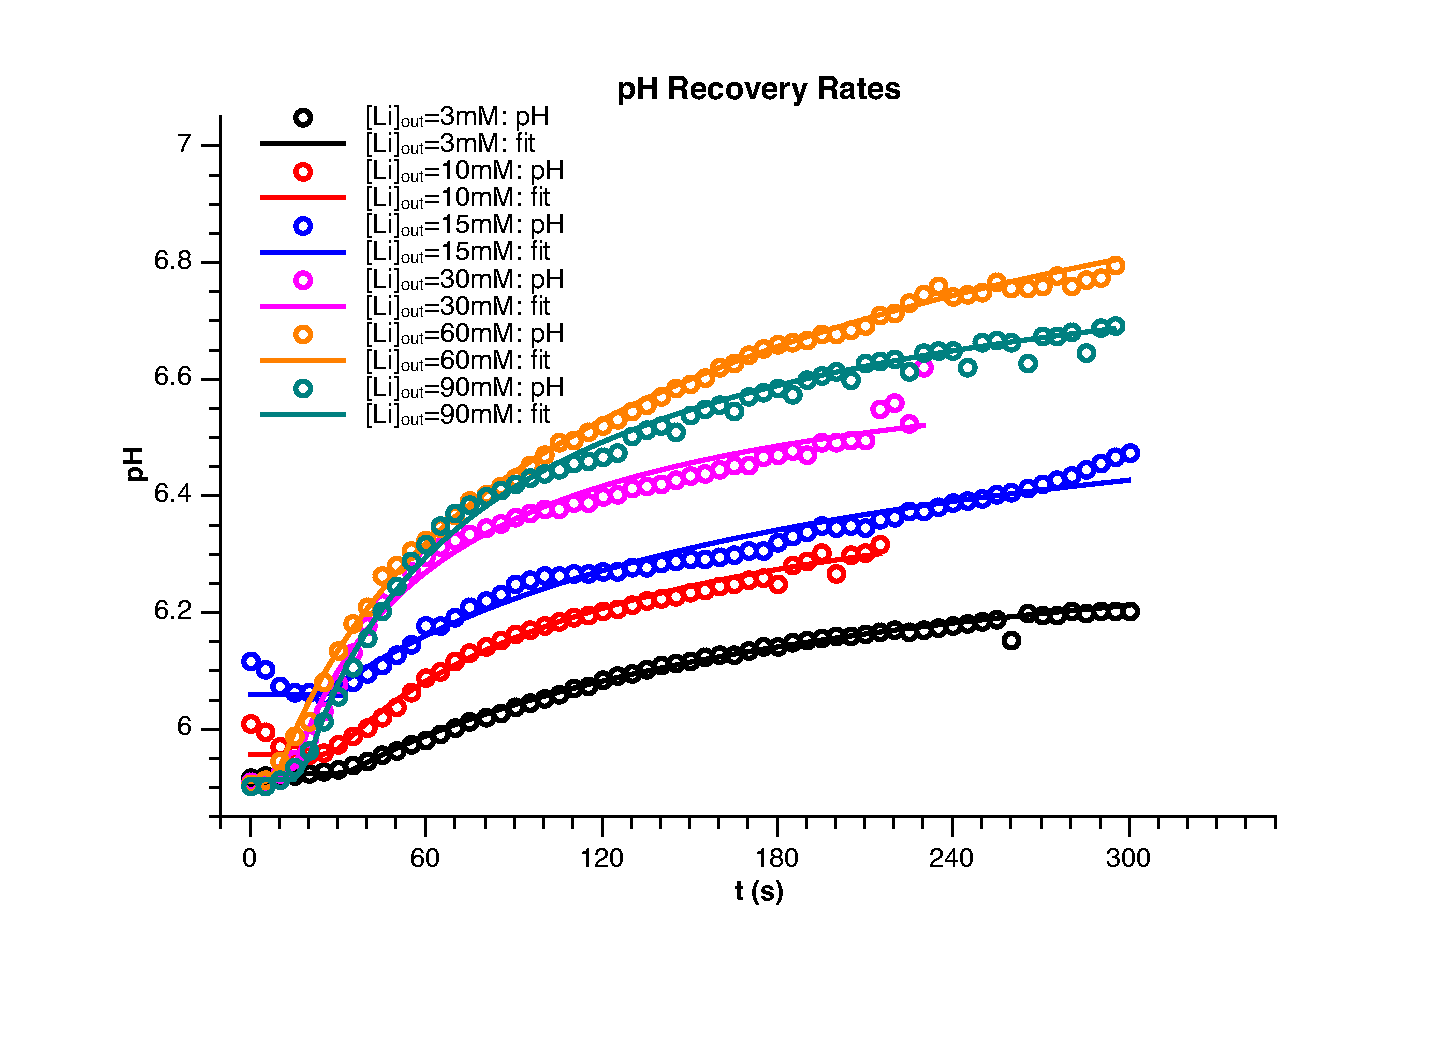
\includegraphics[width=0.75\textwidth]{fig/protons.pdf}
\end{center}
\caption{\label{fig:protons} Fit (lines, according to Eq. \eqref{eq:hfit}) of apparent experimental protons intake (open circles).}
\end{figure}

\subsection{Information from another work about proton recycling}
The proton exit rate by $\NHE{1}$ was studied elsewhere \todo{ref EMBO Lacroix,Counillon}, and this rate depends itself on the inner pH.
From the data presented in figure 3a of that manuscript which shows that the $\NHE{1}$ turnover rate with $\proton$ is a sigmoid function, we
assume:
\begin{equation}
\label{eq:kh}
\left\lbrace
\begin{array}{rcl}
k_h & = & k_0 \eta(h)\\
\eta(h) & \approx & \dfrac{\left(\frac{h}{h_\eta}\right)^{p_\eta}}{1+\left(\frac{h}{h_\eta}\right)^{p_\eta}} \approx 
        \dfrac
{
10^{p_\eta(\mathrm{pH}_\eta-\mathrm{pH})}
}
{
1+10^{p_\eta(\mathrm{pH}_\eta-\mathrm{pH})}
}\\
h_\eta & = & 4\,10^{-7} \; \text{M}\\
\mathrm{pH}_\eta & = & 6.39 \\
p_\eta & = & 1.7 \\
\end{array}
\right.
\end{equation}
and we note that:
\begin{equation}
	\eta'(h) = \left(\dfrac{p_\eta}{h}\right) \dfrac{\left(\frac{h}{h_\eta}\right)^{p_\eta}}{\left[1+\left(\frac{h}{h_\eta}\right)^{p_\eta}\right]^2}  > 0
\end{equation}


\end{document}


